\section{Homework 2} 
\begin{prob}
    Let $E$ and $F$ be any two events. If $P[E] = P[F] = \frac{2}{3}$, then $E$ and $F$ cannot be mutually exclusive. T/F, and why?
\end{prob}
\begin{solution}
    True. If $E,F$ were mutually exclusive, then $P(E \cup F)=P(E)+P(F)= 4/3$. This is a contradiction since probabilities cannot exceed one.
\end{solution}

\begin{prob}
    If events $A$ and $B$ are mutually exclusive, they are necessarily independent. T/F and why?
\end{prob}
\begin{solution}
    True. In general, we have $P(A \cup B)=P(A)+P(B)+P(A\cap B)$. If $A,B$ are mutually exclusive, then \[
        P(A\cup B)=P(A) +P(B)=P(A )+P(B)+P(A \cap B).
    \] This implies that $P(A \cap B)=0$, and the events are necessarily independent.
\end{solution}
\begin{prob}
    A test is used to determine whether people exhibiting green spots have the \emph{duckpox} or not. It is believed that at any given time 4\% of the people exhibiting green spots actually have the \emph{duckpox}. The test is 99\% accurate if a person actually has the \emph{duckpox}. The test is 96\% accurate if a person does \textbf{not} have the \emph{duckpox}. What is the probability that a randomly selected person who tests positive for the \emph{duckpox} actually has the \emph{duckpox}?
\end{prob}
\begin{solution}
    The probability that someone randomly selected tests positive for duckpox is 50.77\%. See the image attached for work. 
    \begin{figure}[H]
    \centering
     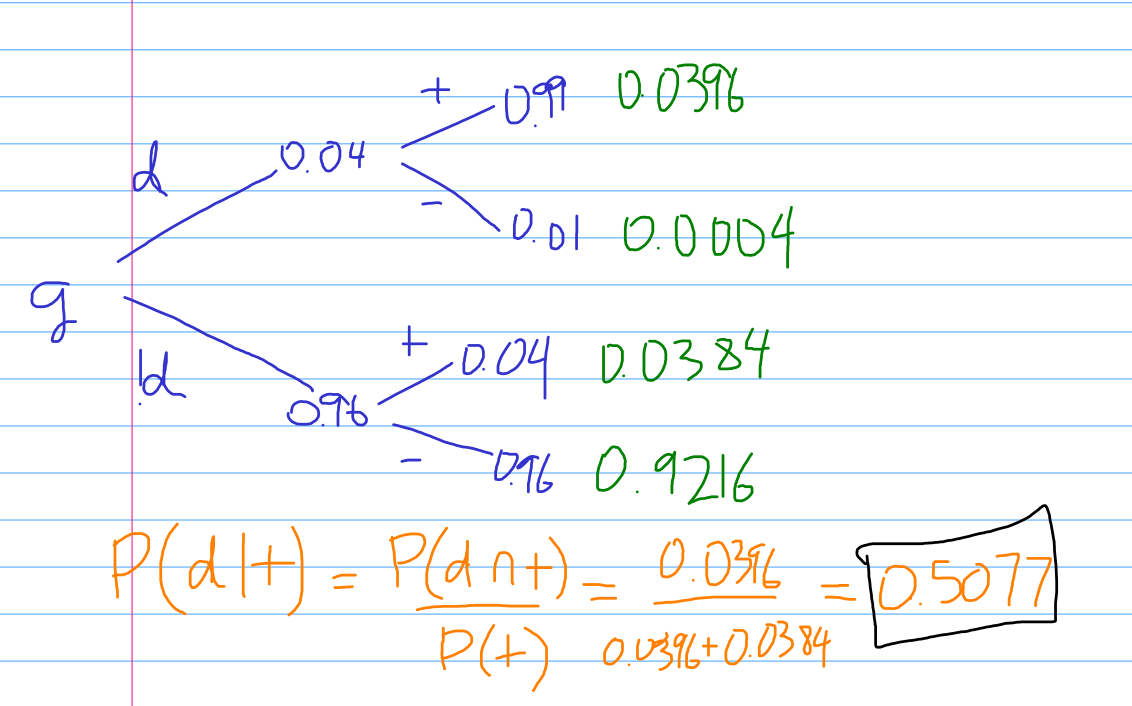
\includegraphics[width=0.6\linewidth]{hw_figures/hw2_duckpox.png}
    \caption{Probability of someone randomly tested having duckpox.}
    \label{hw2_duckpox}
    \end{figure}
\end{solution}
\begin{prob}
    Problem 4.18 as in the textbook.
\end{prob}
\begin{solution}
    \begin{enumerate}[label=(\alph*)]
    \setlength\itemsep{-.2em}
        \item Yes. Each adult is a trial with constant probability of success $p=0.9$, and there are 100 independent trials. 
        \item  The probability that 97 out of 100 sampled Americans had chickenpox is given by \[
                {100\choose 97} (0.9)^{97}(0.1)^3=0.0059.
        \] 
    \item The probability that 3 out of 100 sampled Americans have \emph{not} had chickenpox is given by \[
            {100 \choose 3} (0.1)^3(0.9)^{97}={100\choose 97} (0.9)^{97}(0.1)^3=0.0059.
    \] 
\item The probability that 1 in 10 sampled Americans have had chickenpox is \[
        {10 \choose 1} (0.9)^1(0.1)^{9}=9\cdot 10^{-9}.
    \] 
\item The probability that 3 in 10 sampled Americans have \emph{not} had chickenpox is \[
        {10 \choose 3} (0.1)^{3}(0.9)^{7}=0.0574.
\] 
    \end{enumerate}
\end{solution}

\begin{prob}
    Problem 4.22 as in the textbook.
\end{prob}
\begin{solution}
     We have $n=10$,  $p=0.07$.
     \begin{enumerate}[label=(\alph*)]
     \setlength\itemsep{-.2em}
\item  Here the number of scenarios where at least one has arachnaphobia is $2 ^{10}-1=1023$, since this holds in every scenario except the one where no one has arachnaphobia. So the probability of at least one having arachnaphobia is given by \[
        \sum _{i=1}^{10}\mathrm{Binom}(i, 10, 0.07)=0.516.
\] 
\item This is given by \[
        \mathrm{Binom}(2, 10, 0.07)=0.123.
\] 
\item This is given by \[
        \mathrm{Binom}(0, 10, 0.07)+\mathrm{Binom}(1, 10, 0.07)=0.848.
\] 
\item Yes, the probability is pretty high (more than 80\%).
     \end{enumerate}
\end{solution}

\begin{prob}
    Problem 4.24 as in the textbook.
\end{prob}
\begin{solution}
    We have $n=3$.
    \begin{enumerate}[label=(\alph*)]
    \setlength\itemsep{-.2em}
\item Here $k=2, p=0.25.$ This is given by  $\mathrm{Binom}(2,3,0.25)=0.141$.
\item Here $k=0, p=0.25$. This is given by  $\mathrm{Binom}(0,3,0.25)=0.422$.
\item This is given by \[
        \mathrm{Binom}(1,3,0.25)+\mathrm{Binom}(2,3,0.25)+\mathrm{Binom}(3,3,0.25)=0.578.
    \] 
\item There is one scenario in which this happens, so the probability is given by $1 \cdot (0.25)^1 \cdot (0.75)^2=0.141$.
    \end{enumerate}
\end{solution}
\begin{prob}
    Problem 4.26 as in the book.
\end{prob}
\begin{solution}
    We have $n=3, p=0.51$.
     \begin{enumerate}[label=(\alph*)]
    \setlength\itemsep{-.2em}
\item Here $k=2$. This is given by  $\mathrm{Binom}(2,3,0.51)=0.382$.
\item All possible orderings of two boys in three children are as follows: \[
\begin{tabular}{c|ccc} 
    1 & B & B & G \\ \hline
    2 & B & G & B \\ \hline
    3 & G & B & B
\end{tabular}
\] There are three possibilites. Then the probility of two boys in three children is given by \[
3 \cdot (0.51)^2 \cdot (0.49)=0.382,
\] which matches up with the answer from (a).
\item This would be a lot harder since we would need to write out ${8 \choose 3} =56$ possibilities, which is a lot harder than writing out three possibilities. Therefore it is much easier to use the binomial distribution calculation.
    \end{enumerate}
\end{solution}
